%% LyX 2.3.6 created this file.  For more info, see http://www.lyx.org/.
%% Do not edit unless you really know what you are doing.
\documentclass[english]{article}
\usepackage[T1]{fontenc}
\usepackage[latin9]{inputenc}
\usepackage{amsmath}
\usepackage{graphicx}

\makeatletter

%%%%%%%%%%%%%%%%%%%%%%%%%%%%%% LyX specific LaTeX commands.
%% Because html converters don't know tabularnewline
\providecommand{\tabularnewline}{\\}

\makeatother

\usepackage{babel}
\begin{document}
\title{Towards an ideal Particle Swarm Optimizer for multidimensional functions}
\author{Vasileios Charilogis, Ioannis G. Tsoulos}
\date{Department of Informatics and Telecommunications, University of Ioannina,
Greece}
\maketitle
\begin{abstract}
The Particle Swarm Optimization (PSO) method is a global optimization
technique based on the gradual evolution of a population of solutions
called particles. The method evolves the particles based on both the
best position of each of them in the past and the best position of
the whole. Due to its simplicity, the method has found application
in many scientific areas and for this reason during the last years
many modifications have been presented. This paper introduces three
modifications of the method that aim to reduce the required number
of function calls while maintaining the accuracy of the method in
locating the global minimum. These modifications affect important
components of the method such as how fast the particles change or
even how the method is terminated. The above modifications were tested
on a number of known universal optimization problems from the relevant
literature and the results were compared with similar techniques. 
\end{abstract}

\paragraph*{Keywords:}

Optimization, Evolutionary techniques, Stochastic methods, Termination
rules

\section{Introduction }

The global optimization problem is usually defined as: 
\begin{equation}
x^{*}=\mbox{arg}\min_{x\in S}f(x)\label{eq:eq1}
\end{equation}
with $S$: 
\[
S=\left[a_{1},b_{1}\right]\otimes\left[a_{2},b_{2}\right]\otimes\ldots\left[a_{n},b_{n}\right]
\]
The function $f$ is considered continuous and differentiable function
formulated as $f:S\rightarrow R,S\subset R^{n}$. This problem finds
application in a variety of objective problems from the real world
such as problems of physics \cite{go_physics1,go_physics2,go_physics3},
chemistry \cite{go_chem1,go_chem2,go_chem3}, economics \cite{go_econ1,go_econ2},
medicine \cite{go_med1,go_med2} etc. Global optimization methods
are grouped into two broad categories:\textbf{ }deterministic and
stochastic methods. The most common methods of the first category
are the so called Interval methods \cite{interval1,interval2}, where
the set $S$ is divided iteratively in subregions and some subregions
that not contain the global solution are discarded using some pre
defined criteria. In stochastic methods, the finding of the global
minimum is guided by randomness. In these methods there is no guarantee
to find the global minimum but they constitute the vast majority of
global optimization methods, mainly due to the simplicity in their
implementation. There have been proposed many stochastic methods by
various researchers such as\textbf{ }Controlled Random Search methods
\cite{crs1,crs2,crs3}, Simulated Annealing methods \cite{simann_major,simann1,simann2},\textbf{
}Differential Evolution methods \cite{diffe1,diffe2}, Particle Swarm
Optimization methods \cite{pso_major,pso1,pso2}, Ant Colony Optimization
\cite{aco1,aco2}, Genetic algorithms \cite{ga1,ga2,ga3} etc. Also,
many works have been appeared utilizing the modern GPU processing
units \cite{gpu1,gpu2,gpu3}.

The method of Particle Swarm Optimization is method based on a population
of candidate solutions that called also particles. These particles
have two basic characteristics: their position at any given time\textbf{
$\overrightarrow{x}$} and the speed \textbf{$\overrightarrow{u}$}
at which they move. The purpose of the method is to move the particles
repetitively and their next position is calculated as a function not
only of their position but also of the best position they had in the
past as well as the best position of the population. The method was
successfully used in a variety of scientific and practical problems
from areas such as physics\textbf{ }\cite{psophysics1,psophysics2},
chemistry \cite{psochem1,psochem2}, medicine \cite{psomed1,psomed2},
economics \cite{psoecon} etc. Due to its high popularity, the method
has received a number of interventions in recent years, such as combination
with the mutation mechanism \cite{pso_mutation1,pso_mutation2,pso_mutation3},
improved initialization of the velocity vector \cite{pso_initvelocity},\textbf{
}hybrid techniques \cite{psohybrid1,psohybrid2}, parallel techniques
\cite{pso_parallel1,pso_parallel2,pso_parallel3}, methods aim to
improve the velocity calculation \cite{pso_velocity1,pso_velocity2,pso_velocity3}
etc. This text introduces three distinct modifications to the original
method, which drastically improve the time required to find the total
minimum by reducing the required number of function evaluations. These
modifications cover a large part of the method: the speed calculation,
a new method of avoiding running local search methods and a new adaptive
termination rule. The proposed modifications were applied to a number
of problems from the relevant literature and compared with similar
techniques and the results are presented in a separate section. 

The rest of this article is divided as follows: in section \ref{sec:Method-description}
the initial method and the proposed modifications are discussed, in
section \ref{sec:Experiments} the experiments are listed and finally
in section \ref{sec:Conclusions} some conclusions and guidelines
for future improvements are presented.

\section{Method description \label{sec:Method-description}}

The base algorithm of PSO and the proposed modifications are outlined
in detail in the following subsections. The discussion starts with
a new mechanism that calculates the velocity of the populations, continuous
with a discarding procedure used minimize the number of local searches
performed and ends with a discussion about the new stopping rule proposed
here.

\subsection{The base algorithm\label{subsec:The-base-algorithm}}

The base algorithm is listed below with the periodical application
of local search method in order to enhance the estimation of the global
minimum, ie. at every iteration a decision with probability $p_{l}$
is made in order to apply a local search procedure to some of the
particles. Usually, this probability is small for example 0.05 (5\%).
\begin{enumerate}
\item \textbf{Initialization}. 

\begin{enumerate}
\item \textbf{Set} $\text{\mbox{iter}}=0$ (iteration counter).
\item \textbf{Set} the number of particles $m$.
\item \textbf{Set} the maximum number of iterations allowed $\mbox{iter}_{\mbox{max}}$
\item \textbf{Set} the local search rate $p_{l}\in[0,1]$.
\item \textbf{Initialize} randomly the positions of the $m$ particles $x_{1},x_{2},...,x_{m}$,
with $x_{i}\in S\subset R^{n}$
\item \textbf{Initialize} randomly the velocities of the $m$ particles
$u_{1},u_{2},...,u_{m}$, with $u_{i}\in S\subset R^{n}$
\item \textbf{For} $i=1..m$ do $p_{i}=x_{i}$. The $p_{i}$ vector are
the best located values for every particle $i$.
\item \textbf{Set} $p_{\mbox{best}}=\arg\min_{i\in1..m}f\left(x_{i}\right)$
\end{enumerate}
\item \textbf{Termination Check}.\label{enu:Check-Termination.} Check for
termination. If termination criteria are met then stop.
\item \textbf{For} $i=1..m$ \textbf{Do\label{enu:For}}

\begin{enumerate}
\item \textbf{Update} the velocity $u_{i}$ as a function of $u_{i},\ p_{i}$
and $p_{\mbox{best}}$
\item \textbf{Update} the position $x_{i}=x_{i}+u_{i}$
\item \textbf{Set} $r\in[0,1]$ a random number. If $r\le p_{m}$ then $x_{i}=\mbox{LS}\left(x_{i}\right)$,
where $\mbox{LS}(x)$ is a local search procedure.
\item \textbf{Evaluate} the fitness of the particle $i$, $f\left(x_{i}\right)$
\item \textbf{If} $f\left(x_{i}\right)\le f\left(p_{i}\right)$ then $p_{i}=x_{i}$
\end{enumerate}
\item \textbf{End} \textbf{For}
\item \textbf{Set} $p_{\mbox{best}}=\arg\min_{i\in1..m}f\left(x_{i}\right)$
\item \textbf{Set} $\mbox{iter}=\mbox{iter}+1$. \label{enu:update_k}
\item \textbf{Goto} Step \ref{enu:Check-Termination.}
\end{enumerate}

\subsection{Velocity calculation }

The algorithm of subsection \ref{subsec:The-base-algorithm} calculates
at every iteration the new position $x_{i}$ is calculated using the
old position $x_{i}$ and the associated velocity $u_{i}$ according
to the scheme:
\begin{equation}
x_{i}=x_{i}+u_{i}\label{eq:eq3}
\end{equation}
Typically the velocity is calculated as a combination of the old velocity
and the best located values $p_{i}$ and $p_{\mbox{best}}$ and may
be defined as:
\begin{equation}
u_{i}=\omega u_{i}+r_{1}c_{1}\left(p_{i}-x_{i}\right)+r_{2}c_{2}\left(p_{\mbox{best}}-x_{i}\right)\label{eq:eq4-1}
\end{equation}
where 
\begin{enumerate}
\item The parameters $r_{1},\ r_{2}$ are random numbers with $r_{1}\in[0,1]$
and $r_{2}\in[0,1]$.
\item The constant number $c_{1},\ c_{2}$ are in the range $[1,2]$.
\item The variable $\omega$ is called inertia, with $\omega\in[0,1]$. 
\end{enumerate}
The inertia was proposed by Shi and Eberhart \cite{pso_major}. They
argued that high values of the inertia coefficient cause better exploration
of the search area while small values of this variable are used when
we want to achieve better local research around promising areas for
the global minimum. The value of the inertia factor generally starts
with large values and decreases with the repetition. This article
proposes a new adaptive technique for the inertia parameter and it
this mechanism is compared against three others from the relevant
literature.

\subsubsection{Random inertia}

The inertia calculation is proposed in \cite{random_inertia} and
it is defined as
\begin{equation}
\omega_{\mbox{iter}}=0.5+\frac{r}{2}
\end{equation}
where $r$ a random number with $r\in[0,1]$. This inertia calculation
will be called I1 in the tables with the experimental results.

\subsubsection{Linear time varying inertia ( min version)}

This inertia schema has been proposed in used in various studies \cite{random_inertia,inertia1,inertia2}
and it is defined as:
\begin{equation}
\omega_{\mbox{iter}}=\frac{\mbox{iter}_{\mbox{max}}-\mbox{iter}}{\mbox{iter}_{\mbox{max}}}\left(\omega_{\mbox{max}}-\omega_{\mbox{min}}\right)+\omega_{\mbox{min}}
\end{equation}
where $\omega_{min}$ is the minimum value of inertia and $\omega_{\mbox{max}}$
the maximum value for inertia. This inertia calculation will be called
I2 in the tables with the experimental results.

\subsubsection{Linear time varying inertia ( max version )}

This method is proposed in \cite{inertia3,inertia4} and it is defined
as:
\begin{equation}
\omega_{\mbox{iter}}=\frac{\mbox{iter}_{\mbox{max}}-\mbox{iter}}{\mbox{iter}_{\mbox{max}}}\left(\omega_{\mbox{min}}-\omega_{\mbox{max}}\right)+\omega_{\mbox{max}}
\end{equation}
This inertia calculation will be called I3 in the tables with the
experimental results.

\subsubsection{Proposed technique}

This calculation of inertia involves the number of iterations where
the method manages to find a new minimum. In the first iterations
and when the method has to do more exploration of the research area
the inertia will be great. When the method should focus on a minimum,
then the inertia will decrease. For this reason at every iteration
$\mbox{iter}$ the quantity 
\begin{equation}
\text{\ensuremath{\delta^{(\mbox{iter})}=}}\left|\sum_{i=1}^{m}\left|f_{i}^{(\mbox{iter})}\right|-\sum_{i=1}^{m}\left|f_{i}^{(\mbox{iter}-1)}\right|\right|
\end{equation}
is measured. In the first steps of the algorithm this quantity will
change from repetition to repetition at a fast pace and at some point
and then it will no longer change at the same rate or will be zero.
Hence, we define a metric to model the changes in $\delta^{(\mbox{iter})}\ $as
\begin{equation}
\zeta^{(\mbox{iter})}=\begin{cases}
1, & \delta^{(i)}=0\\
0, & \mbox{otherwise}
\end{cases}
\end{equation}
 Using this observation two additional metrics are created, $S_{\delta}^{(\mbox{iter})}$
and $C_{\delta}^{(\mbox{iter})}$. The metric $S_{\delta}^{(\mbox{iter})}$
is given by
\begin{equation}
S_{\delta}^{(\mbox{iter})}=\sum_{i=1}^{\mbox{iter}}\zeta^{(i)}
\end{equation}
and the metric $C_{\delta}$ is given by:
\begin{equation}
C_{\delta}^{(\mbox{iter})}=\frac{S_{\delta}^{(\mbox{iter)}}}{\mbox{iter}}
\end{equation}
The following definition for the inertia calculation is proposed:
\begin{equation}
\omega_{\mbox{iter}}=\omega_{max}-\frac{\mbox{iter}}{C_{\delta}^{(\mbox{iter})}}\left(\omega_{\mbox{max}}-\omega_{\mbox{min}}\right)\label{eq:proposedInertia}
\end{equation}
This mechanism will be called IP in the tables with the experimental
results.

\subsection{The discarding procedure}

The method in each iteration performs under conditional a series of
local searches. However, these searches will often either lead to
local minima already found or locate values far below the global minimum.
This means that much of the computing time will be wasted on actions
that could have been avoided. In order to be able to group points
that would lead by local search to the same local minimum, we introduce
the concept of cluster, which refers to a set of points that are believed,
under some asymptotic considerations, to belong to the same region
of attraction of the function. The region of attraction for a local
minimum $x^{*}$ is defined as:
\begin{equation}
A\left(x^{*}\right)=\left\{ x:\ x\in S\subset R^{n},\ \mbox{LS}(x)=x^{*}\right\} 
\end{equation}
 where $\mbox{LS}(x)$ is a local search procedure that starts from
a given point $x$ and terminates when a local minimum is discovered.
The discarding procedure suggested here prevents the method from starting
a local search from a point $x$ if that point belongs to the same
region of attraction with other points. This procedure is composed
by two two major parts:
\begin{enumerate}
\item The first part is the so called typical distance, which is a measure
calculated after every local search and it is given by 
\begin{equation}
r_{C}=\frac{1}{M}\sum_{i=1}^{M}\left\Vert x_{i}-x_{iL}\right\Vert \label{eq:eq2}
\end{equation}
where the local search procedure $\mbox{LS}(x)$ initiates from $x_{i}$
and $x_{iL}$ is the outcome of $\mbox{LS}\left(x_{i}\right)$. This
measure has been used also in \cite{minfinder}. If a point $x$ is
close enough to an already discovered local minima then it is highly
possible that the point belongs to the so called region of attraction
of the minima.
\item The second part is a check using the gradient values between a candidate
starting point and an already discovered local minimum. The function
value $f(x)$ near to some local minimum $z$ can be calculated using:
\begin{equation}
f(x)\simeq f(z)+\frac{1}{2}\left(x-z\right)^{T}B\left(x-z\right)\label{eq:eq4}
\end{equation}
where $B$ is the Hessian matrix at the minimum $z.$ By taking gradients
in both sides of Equation \ref{eq:eq4} we obtain:
\begin{equation}
\nabla f(x)\simeq B\left(x-z\right)\label{eq:eq5}
\end{equation}
Of course equation \ref{eq:eq5} holds for any other point $y$ near
to $z$ 
\begin{equation}
\nabla f(y)\simeq B\left(y-z\right)\label{eq:eq6}
\end{equation}
By subtracting the equation $\ref{eq:eq6}$ from \ref{eq:eq5} and
by multiplying with $\left(x-y\right)^{T}$ we have the following
equation:
\begin{equation}
\left(x-y\right)^{T}\left(\nabla f(x)-\nabla f(y)\right)\simeq\left(x-y\right)^{T}B\left(x-y\right)^{T}>0\label{eq:eq7}
\end{equation}
\end{enumerate}
Hence, a candidate start point $x$ can be rejected if 
\begin{equation}
\left\Vert x-z\right\Vert \le r_{C}\ \mbox{AND\ }\left(x-y\right)^{T}\left(\nabla f(x)-\nabla f(z)\right)\label{eq:gradientCheck}
\end{equation}
 for any already discovered local minimum $z$.

\subsection{Stopping rule}

A common used way to terminate a global optimization method is to
utilize a maximum number of allowed iterations $\mbox{iter}_{\mbox{max}}$,
i.e. stop when $\mbox{iter}\ge\mbox{iter}_{\mbox{max}}$. Although,
it is a simple criterion but is not an efficient one since, if $\mbox{iter}_{\mbox{max}}$
is tool small, then the algorithm will terminate without locating
the global optimum. Also, when $\mbox{iter}_{\mbox{max}}$ is too
high, the optimization algorithm will spend computation time in unnecessary
function calls. In this paper a new termination rule is proposed to
terminate the PSO process and it is compared against two other methods
used in various optimization methods.

\subsubsection{Ali's stopping method}

A method proposed in the work of Ali and Kaelo\cite{AliKaelo}, where
at every generation the measure 
\begin{equation}
\alpha=\left|f_{\mbox{max}}-f_{\mbox{min}}\right|
\end{equation}
 is calculated. The $f_{\mbox{max}}$ stands for the maximum function
value of the population and $f_{\mbox{min}}$ represents the lowest
function value of the population. The method will terminate when
\begin{equation}
\alpha\le\epsilon\label{eq:termination_ali}
\end{equation}
where $\epsilon$ is a predefined small positive value, for example
$\epsilon=10^{-3}$.

\subsubsection{Doublebox method }

The second method utilized is a method initially proposed \cite{doublepop_tsoulos}.
In this method we denote with\textbf{ $\sigma^{(iter)}$ }the variance
of $f_{\mbox{min}}$ calculated at iteration $\mbox{iter}$. If the
algorithm can not locate a new lower value for $f_{\mbox{min}}$\textbf{
}for a number of iterations, then the global minimum has already located
and the algorithm should terminate, i.e. terminate when\textbf{ }

\begin{equation}
\sigma^{(\mbox{iter})}\le\frac{\sigma^{\left(\mbox{iter}_{\mbox{last}}\right)}}{2}\label{eq:termination_doublebox}
\end{equation}
where $\mbox{iter}_{\mbox{last}}$ stands for the last iteration where
a new lower value for $f_{\mbox{min}}$was discovered.

\subsubsection{Proposed technique}

In the proposed termination technique in each iteration $\mbox{k}$
the difference between the current best value and the previous best
value is measured, ie the difference $\left|f_{\mbox{min}}^{(k)}-f_{\mbox{min}}^{(k-1)}\right|.$
If this difference is zero for a series of predefined number of iterations
$k_{\mbox{max}}$, then the method terminates. 

\section{Experiments \label{sec:Experiments}}

To measure the effect of the proposed modifications on the original
method, a series of experiments were performed on test functions from
the relevant literature. \cite{Ali1,Floudas1} and they have been
used widely by various researchers \cite{testfunctions1,testfunctions2,testfunctions3,testfunctions4}.
The experiments evaluated both the effect of the new method of calculating
inertia, as well as the criterion for avoiding local minima as well
as the new termination rule. The experiments were recorded in separate
tables, so that it is more possible to understand the effect of each
modification separately. 

\subsection{Test functions}

The definition of the test functions used are given below
\begin{itemize}
\item \textbf{Bf1} (Bohachevsky 1) function:
\end{itemize}
\[
f(x)=x_{1}^{2}+2x_{2}^{2}-\frac{3}{10}\cos\left(3\pi x_{1}\right)-\frac{4}{10}\cos\left(4\pi x_{2}\right)+\frac{7}{10}
\]
with $x\in[-100,100]^{2}$. 
\begin{itemize}
\item \textbf{Bf2} (Bohachevsky 2) function: 
\[
f(x)=x_{1}^{2}+2x_{2}^{2}-\frac{3}{10}\cos\left(3\pi x_{1}\right)\cos\left(4\pi x_{2}\right)+\frac{3}{10}
\]
with $x\in[-50,50]^{2}$. 
\item \textbf{Branin} function: $f(x)=\left(x_{2}-\frac{5.1}{4\pi^{2}}x_{1}^{2}+\frac{5}{\pi}x_{1}-6\right)^{2}+10\left(1-\frac{1}{8\pi}\right)\cos(x_{1})+10$
with $-5\le x_{1}\le10,\ 0\le x_{2}\le15$. with $x\in[-10,10]^{2}$. 
\item \textbf{CM} function: 
\[
f(x)=\sum_{i=1}^{n}x_{i}^{2}-\frac{1}{10}\sum_{i=1}^{n}\cos\left(5\pi x_{i}\right)
\]
where $x\in[-1,1]^{n}$. In the current experiments we used $n=4$.
\item \textbf{Camel} function:
\[
f(x)=4x_{1}^{2}-2.1x_{1}^{4}+\frac{1}{3}x_{1}^{6}+x_{1}x_{2}-4x_{2}^{2}+4x_{2}^{4},\quad x\in[-5,5]^{2}
\]
\item \textbf{Easom} function: 
\[
f(x)=-\cos\left(x_{1}\right)\cos\left(x_{2}\right)\exp\left(\left(x_{2}-\pi\right)^{2}-\left(x_{1}-\pi\right)^{2}\right)
\]
with $x\in[-100,100]^{2}.$ 
\item \textbf{Exponential} function, defined as: 
\[
f(x)=-\exp\left(-0.5\sum_{i=1}^{n}x_{i}^{2}\right),\quad-1\le x_{i}\le1
\]
 In the current experiments we used this function with $n=2,4,8,16,32$.
\item \textbf{Goldstein and Price function }\\
\begin{eqnarray*}
f(x) & = & \left[1+\left(x_{1}+x_{2}+1\right)^{2}\right.\\
 &  & \left(19-14x_{1}+3x_{1}^{2}-14x_{2}+6x_{1}x_{2}+3x_{2}^{2}\right)]\times\\
 &  & [30+\left(2x_{1}-3x_{2}\right)^{2}\\
 &  & \left(18-32x_{1}+12x_{1}^{2}+48x_{2}-36x_{1}x_{2}+27x_{2}^{2}\right)]
\end{eqnarray*}
With $x\in[-2,2]^{2}$. 
\item \textbf{Griewank2} function:
\[
f(x)=1+\frac{1}{200}\sum_{i=1}^{2}x_{i}^{2}-\prod_{i=1}^{2}\frac{\cos(x_{i})}{\sqrt{(i)}},\quad x\in[-100,100]^{2}
\]
\item \textbf{Gkls} function. $f(x)=\mbox{Gkls}(x,n,w)$, is a function
with $w$ local minima, described in \cite{gkls} with $x\in[-1,1]^{n}$
and $n$ a positive integer between 2 and 100. The value of the global
minimum is -1 and in our experiments we have used $n=2,3$ and $w=50,\ 100$. 
\item \textbf{Hansen} function: $f(x)=\sum_{i=1}^{5}i\cos\left[(i-1)x_{1}+i\right]\sum_{j=1}^{5}j\cos\left[(j+1)x_{2}+j\right]$,
$x\in[-10,10]^{2}$ .
\item \textbf{Hartman 3} function:
\[
f(x)=-\sum_{i=1}^{4}c_{i}\exp\left(-\sum_{j=1}^{3}a_{ij}\left(x_{j}-p_{ij}\right)^{2}\right)
\]
with $x\in[0,1]^{3}$ and $a=\left(\begin{array}{ccc}
3 & 10 & 30\\
0.1 & 10 & 35\\
3 & 10 & 30\\
0.1 & 10 & 35
\end{array}\right),\ c=\left(\begin{array}{c}
1\\
1.2\\
3\\
3.2
\end{array}\right)$ and
\[
p=\left(\begin{array}{ccc}
0.3689 & 0.117 & 0.2673\\
0.4699 & 0.4387 & 0.747\\
0.1091 & 0.8732 & 0.5547\\
0.03815 & 0.5743 & 0.8828
\end{array}\right)
\]
\item \textbf{Hartman 6} function:
\[
f(x)=-\sum_{i=1}^{4}c_{i}\exp\left(-\sum_{j=1}^{6}a_{ij}\left(x_{j}-p_{ij}\right)^{2}\right)
\]
with $x\in[0,1]^{6}$ and $a=\left(\begin{array}{cccccc}
10 & 3 & 17 & 3.5 & 1.7 & 8\\
0.05 & 10 & 17 & 0.1 & 8 & 14\\
3 & 3.5 & 1.7 & 10 & 17 & 8\\
17 & 8 & 0.05 & 10 & 0.1 & 14
\end{array}\right),\ c=\left(\begin{array}{c}
1\\
1.2\\
3\\
3.2
\end{array}\right)$ and
\[
p=\left(\begin{array}{cccccc}
0.1312 & 0.1696 & 0.5569 & 0.0124 & 0.8283 & 0.5886\\
0.2329 & 0.4135 & 0.8307 & 0.3736 & 0.1004 & 0.9991\\
0.2348 & 0.1451 & 0.3522 & 0.2883 & 0.3047 & 0.6650\\
0.4047 & 0.8828 & 0.8732 & 0.5743 & 0.1091 & 0.0381
\end{array}\right)
\]
\item \textbf{Potential} function. The molecular conformation corresponding
to the global minimum of the energy of N atoms interacting via the
Lennard-Jones potential\cite{Jones} is used a test function here
and it is defined by:
\begin{equation}
V_{LJ}(r)=4\epsilon\left[\left(\frac{\sigma}{r}\right)^{12}-\left(\frac{\sigma}{r}\right)^{6}\right]\label{eq:potential}
\end{equation}
For our experiments we used: $N=3,\ 4,\ 5$
\item \textbf{Rastrigin} function. 
\[
f(x)=x_{1}^{2}+x_{2}^{2}-\cos(18x_{1})-\cos(18x_{2}),\quad x\in[-1,1]^{2}
\]
\item \textbf{\emph{Rosenbrock}}\emph{ function}.\\
\[
f(x)=\sum_{i=1}^{n-1}\left(100\left(x_{i+1}-x_{i}^{2}\right)^{2}+\left(x_{i}-1\right)^{2}\right),\quad-30\le x_{i}\le30.
\]
In our experiments we used the values $n=4,\ 8,\ 16$.
\item \textbf{Shekel 7} function.
\end{itemize}
\[
f(x)=-\sum_{i=1}^{7}\frac{1}{(x-a_{i})(x-a_{i})^{T}+c_{i}}
\]

with $x\in[0,10]^{4}$ and $a=\left(\begin{array}{cccc}
4 & 4 & 4 & 4\\
1 & 1 & 1 & 1\\
8 & 8 & 8 & 8\\
6 & 6 & 6 & 6\\
3 & 7 & 3 & 7\\
2 & 9 & 2 & 9\\
5 & 3 & 5 & 3
\end{array}\right),\ c=\left(\begin{array}{c}
0.1\\
0.2\\
0.2\\
0.4\\
0.4\\
0.6\\
0.3
\end{array}\right)$. 
\begin{itemize}
\item \textbf{Shekel 5 }function.
\end{itemize}
\[
f(x)=-\sum_{i=1}^{5}\frac{1}{(x-a_{i})(x-a_{i})^{T}+c_{i}}
\]
 

with $x\in[0,10]^{4}$ and $a=\left(\begin{array}{cccc}
4 & 4 & 4 & 4\\
1 & 1 & 1 & 1\\
8 & 8 & 8 & 8\\
6 & 6 & 6 & 6\\
3 & 7 & 3 & 7
\end{array}\right),\ c=\left(\begin{array}{c}
0.1\\
0.2\\
0.2\\
0.4\\
0.4
\end{array}\right)$. 
\begin{itemize}
\item \textbf{Shekel 10} function.
\end{itemize}
\[
f(x)=-\sum_{i=1}^{10}\frac{1}{(x-a_{i})(x-a_{i})^{T}+c_{i}}
\]
 

with $x\in[0,10]^{4}$ and $a=\left(\begin{array}{cccc}
4 & 4 & 4 & 4\\
1 & 1 & 1 & 1\\
8 & 8 & 8 & 8\\
6 & 6 & 6 & 6\\
3 & 7 & 3 & 7\\
2 & 9 & 2 & 9\\
5 & 5 & 3 & 3\\
8 & 1 & 8 & 1\\
6 & 2 & 6 & 2\\
7 & 3.6 & 7 & 3.6
\end{array}\right),\ c=\left(\begin{array}{c}
0.1\\
0.2\\
0.2\\
0.4\\
0.4\\
0.6\\
0.3\\
0.7\\
0.5\\
0.6
\end{array}\right)$. 
\begin{itemize}
\item \textbf{Sinusoidal} function: 
\[
f(x)=-\left(2.5\prod_{i=1}^{n}\sin\left(x_{i}-z\right)+\prod_{i=1}^{n}\sin\left(5\left(x_{i}-z\right)\right)\right),\quad0\le x_{i}\le\pi.
\]
The case of $n=4,8,16,32$ and $z=\frac{\pi}{6}$ was used in the
experimental results.
\item \textbf{Test2N} function:
\[
f(x)=\frac{1}{2}\sum_{i=1}^{n}x_{i}^{4}-16x_{i}^{2}+5x_{i},\quad x_{i}\in[-5,5].
\]
The function has $2^{n}$ in the specified range and in our experiments
we used $n=4,5,6,7$.
\item \textbf{Test30N} function:
\[
f(x)=\frac{1}{10}\sin^{2}\left(3\pi x_{1}\right)\sum_{i=2}^{n-1}\left(\left(x_{i}-1\right)^{2}\left(1+\sin^{2}\left(3\pi x_{i+1}\right)\right)\right)+\left(x_{n}-1\right)^{2}\left(1+\sin^{2}\left(2\pi x_{n}\right)\right)
\]
with $x\in[-10,10]$, with $30^{n}$ local minima in the search space.
For our experiments we used $n=3,4$.
\end{itemize}

\subsection{Experimental setup}

All the experiments have been performed 30 times using a different
seed for the random number generator each. The code has been implemented
in ANSI C++ and the well - known function drand48() was used to produce
random numbers. The local search method used as BFGS method\textbf{
}\cite{Powell}.\textbf{ }All the parameters used in the conducted
experiments are listed in Table \ref{tab:parameters}.

\begin{table}
\caption{Values for the experimental parameters.\label{tab:parameters}}

\centering{}%
\begin{tabular}{|c|c|}
\hline 
PARAMETER & VALUE\tabularnewline
\hline 
\hline 
$m$ & 100\tabularnewline
\hline 
$\mbox{iter}_{\mbox{max}}$ & 100\tabularnewline
\hline 
$p_{l}$ & 0.05\tabularnewline
\hline 
$c_{1}$ & 1.0\tabularnewline
\hline 
$c_{2}$ & 1.0\tabularnewline
\hline 
$\omega_{min}$ & 0.4\tabularnewline
\hline 
$\omega_{max}$ & 0.9\tabularnewline
\hline 
$\epsilon$ & 0.001\tabularnewline
\hline 
$k_{\mbox{max}}$ & 15\tabularnewline
\hline 
\end{tabular}
\end{table}


\subsection{Experimental results }

For every stopping rule two tables are listed: the first one contains
experiments with the relevant stopping rule without the gradient discarding
procedure and the second table contains experiments with the gradient
discarding procedure enabled. The numbers in table cells stand for
average function calls. The fraction in parentheses denotes the fraction
of runs where the global optimum was found. Absence of this fractions
means that the global minimum was discovered in every run (100\% success).
The experimental results using the stopping rule of Equation \ref{eq:termination_ali}
are listed in Tables \ref{tab:AliNoGradient} and \ref{tab:AliGradient}.
The experimental results for the Double Box stopping rule of Equation
\ref{eq:termination_doublebox} are listed in Tables \ref{tab:DoubleBoxNoGradient}
and \ref{tab:DoubleBoxWithGradient}. Finally, for the proposed stopping
rule the results are listed in Tables \ref{tab:ProposedNoGradient}
and \ref{tab:ProposedWithGradient}. The above results lead to a number
of observations:
\begin{enumerate}
\item The PSO method is a robust method and this is evident by the high
success rate in finding the global minimum, although the number of
particles used was relative low (100).
\item The proposed inertia calculation method as defined in Equation \ref{eq:proposedInertia}
achieves a significant reduction in the number of calls between 11
and 25\% depending on the termination criterion used. However, the
presence of the gradient check mechanism of the Equation \ref{eq:gradientCheck}
nullifies any gain of the method, as the rejection criterion significantly
reduces the number of calls regardless of the inertia calculation
mechanism used. 
\item The local optimization avoidance mechanism of the gradient check drastically
reduces the required number of calls for each termination criterion
while maintaining the success rate of the method at extremely high
levels. 
\item The proposed termination criterion is significantly superior to the
other two with which the comparison was made. Also, if the termination
criterion is combined with the mechanism for avoiding local optimizations,
then the gain in number of calls grows even more. 
\end{enumerate}
To show the effect of the proposed termination method, an additional
experiment was performed in which the dimension of the sinus problem
increases from 2 to 32 and in each case all three termination techniques
were tested. The result of this experiment is graphically represented
in the Figure \ref{fig:sinu}. This graph shows that the doublebox
method is significantly superior to the ali method but of course the
new proposed method further reduces the required number of function
calls. 

\begin{table}
\caption{Experiments with the Ali stopping rule, without gradient check.\label{tab:AliNoGradient}}

\centering{}%
\begin{tabular}{|c|c|c|c|c|}
\hline 
\textbf{FUNCTION} & \textbf{I1} & \textbf{I2} & \textbf{I3} & \textbf{IP}\tabularnewline
\hline 
\hline 
BF1 & 24929 & 22874 & 18739 & 22088\tabularnewline
\hline 
BF2 & 24043 & 22254 & 17172 & 20743\tabularnewline
\hline 
BRANIN & 17691 & 16205 & 13397 & 12471\tabularnewline
\hline 
CM4 & 20117 & 22568 & 26867 & 14941\tabularnewline
\hline 
CAMEL & 19474 & 17813 & 14461 & 13492\tabularnewline
\hline 
EASOM & 13327 & 13106 & 9969 & 9212\tabularnewline
\hline 
EXP2 & 6339 & 8243 & 7853 & 3501\tabularnewline
\hline 
EXP4 & 7816 & 10066 & 10900 & 4458\tabularnewline
\hline 
EXP8 & 8667 & 10937 & 13126 & 4761\tabularnewline
\hline 
EXP16 & 8748 & 11402 & 15754 & 5098\tabularnewline
\hline 
EXP32 & 9567 & 12323 & 18189 & 5471\tabularnewline
\hline 
GKLS250 & 10907 & 12562 & 9673 & 8552\tabularnewline
\hline 
GKLS2100 & 12960 & 13403 & 9930 & 9541\tabularnewline
\hline 
GKLS350 & 15410(0.97) & 14722 & 10542 & 9298\tabularnewline
\hline 
GKLS3100 & 16639 & 14495 & 10412 & 13075(0.97)\tabularnewline
\hline 
GOLDSTEIN & 20437 & 22877 & 16410 & 8935\tabularnewline
\hline 
GRIEWANK2 & 27620 & 24230 & 18473 & 20133\tabularnewline
\hline 
HANSEN & 21513 & 20279 & 16326 & 15046\tabularnewline
\hline 
HARTMAN3 & 16233 & 17152 & 12305 & 6511\tabularnewline
\hline 
HARTMAN6 & 47038 & 48947 & 46852 & 23431\tabularnewline
\hline 
POTENTIAL3 & 31684 & 32175 & 36930 & 24463\tabularnewline
\hline 
POTENTIAL4 & 184602 & 181231 & 168962 & 129267\tabularnewline
\hline 
POTENTIAL5 & 74508 & 70519 & 76890 & 54042\tabularnewline
\hline 
RASTRIGIN & 23574 & 20865 & 15596 & 16198\tabularnewline
\hline 
ROSENBROCK4 & 145178 & 161136 & 160341 & 129891\tabularnewline
\hline 
ROSENBROCK8 & 95290 & 97035 & 96687 & 80408\tabularnewline
\hline 
ROSENBCROK16 & 118614 & 116454 & 115122 & 97004\tabularnewline
\hline 
SHEKEL5 & 27458 & 27088 & 25927 & 18036\tabularnewline
\hline 
SHEKEL7 & 27521 & 27271 & 25967 & 18805\tabularnewline
\hline 
SHEKEL10 & 29699(0.97) & 28082 & 25511 & 20823\tabularnewline
\hline 
TEST2N4 & 26740 & 27050 & 22905 & 19495\tabularnewline
\hline 
TEST2N5 & 20243(0.97) & 20290 & 17729 & 16024(0.97)\tabularnewline
\hline 
TEST2N6 & 33118 & 33366 & 30118 & 25235(0.93)\tabularnewline
\hline 
TEST2N7 & 23266(0.90) & 22804 & 21294 & 18218(0.90)\tabularnewline
\hline 
SINU4 & 17035 & 20487 & 18971 & 11079\tabularnewline
\hline 
SINU8 & 22827 & 27176 & 27732 & 12379\tabularnewline
\hline 
SINU16 & 31055 & 35998 & 42984 & 15692\tabularnewline
\hline 
SINU32 & 44736(0.97) & 51624 & 82114 & 25991\tabularnewline
\hline 
TEST30N3 & 18733 & 20119 & 17803 & 17543\tabularnewline
\hline 
TEST30N4 & 20348 & 22191 & 20679 & 20085\tabularnewline
\hline 
\textbf{TOTAL} & 1365704(0.99) & 1399419 & 1367612 & 1001436(0.99)\tabularnewline
\hline 
\end{tabular}
\end{table}

\begin{table}
\caption{Experiments with the Ali stopping rule, with the gradient check enabled.\label{tab:AliGradient}}

\centering{}%
\begin{tabular}{|c|c|c|c|c|}
\hline 
\textbf{FUNCTION} & \textbf{I1} & \textbf{I2} & \textbf{I3} & \textbf{IP}\tabularnewline
\hline 
\hline 
BF1 & 9709 & 8918 & 9531 & 10932\tabularnewline
\hline 
BF2 & 10196 & 9588 & 9089 & 10730\tabularnewline
\hline 
BRANIN & 10718 & 9597 & 9813 & 9501\tabularnewline
\hline 
CM4 & 6242 & 7503 & 12531 & 6985\tabularnewline
\hline 
CAMEL & 10422 & 9306 & 8491 & 9624\tabularnewline
\hline 
EASOM & 11565 & 11366 & 8497 & 8196\tabularnewline
\hline 
EXP2 & 3364 & 4443 & 4558 & 1926\tabularnewline
\hline 
EXP4 & 3558 & 4767 & 6023 & 2122\tabularnewline
\hline 
EXP8 & 3716 & 4787 & 7753 & 2186\tabularnewline
\hline 
EXP16 & 3784 & 5076 & 9696 & 2211\tabularnewline
\hline 
EXP32 & 4137 & 5698 & 11379 & 2323\tabularnewline
\hline 
GKLS250 & 5917 & 7080 & 7517 & 5273\tabularnewline
\hline 
GKLS2100 & 6843 & 8261 & 7449 & 7296\tabularnewline
\hline 
GKLS350 & 6845 & 8076 & 7833 & 5881(0.97)\tabularnewline
\hline 
GKLS3100 & 10290(0.93) & 10187 & 7828 & 8066(0.97)\tabularnewline
\hline 
GOLDSTEIN & 7977 & 9035 & 8505 & 4381\tabularnewline
\hline 
GRIEWANK2 & 12567 & 12222 & 12000 & 12037\tabularnewline
\hline 
HANSEN & 13441 & 13360 & 11876 & 10818\tabularnewline
\hline 
HARTMAN3 & 9758 & 9548 & 8123 & 4114\tabularnewline
\hline 
HARTMAN6 & 12893(0.90) & 12889(0.93) & 22309 & 10126(0.93)\tabularnewline
\hline 
POTENTIAL3 & 17912 & 16420 & 21904 & 15969\tabularnewline
\hline 
POTENTIAL4 & 73629 & 64886 & 95707 & 67084\tabularnewline
\hline 
POTENTIAL5 & 40585 & 35239 & 47807 & 33661\tabularnewline
\hline 
RASTRIGIN & 11305 & 10101 & 11141 & 10046\tabularnewline
\hline 
ROSENBROCK4 & 18115 & 21919 & 38407 & 43093\tabularnewline
\hline 
ROSENBROCK8 & 12869 & 14192 & 31923 & 25405\tabularnewline
\hline 
ROSENBCROK16 & 12096 & 13023 & 38486 & 23165\tabularnewline
\hline 
SHEKEL5 & 10347 & 11466 & 14446 & 11802\tabularnewline
\hline 
SHEKEL7 & 11511 & 10521 & 13944 & 10399\tabularnewline
\hline 
SHEKEL10 & 10834 & 10842 & 13785 & 12253\tabularnewline
\hline 
TEST2N4 & 11133 & 10869 & 12161 & 11546\tabularnewline
\hline 
TEST2N5 & 10923(0.97) & 10315 & 10868 & 11072(0.97)\tabularnewline
\hline 
TEST2N6 & 12331(0.97) & 12345 & 14123 & 15652\tabularnewline
\hline 
TEST2N7 & 11342(0.93) & 11354 & 12118 & 12370(0.93)\tabularnewline
\hline 
SINU4 & 7724 & 9845 & 12294 & 6575\tabularnewline
\hline 
SINU8 & 8468 & 10969 & 18122 & 5382\tabularnewline
\hline 
SINU16 & 9334 & 13213 & 31589 & 9294\tabularnewline
\hline 
SINU32 & 13290 & 17502(0.97) & 63111(0.97) & 14959\tabularnewline
\hline 
TEST30N3 & 12675 & 12954 & 12472 & 12482\tabularnewline
\hline 
TEST30N4 & 13964 & 14903 & 14999 & 15389\tabularnewline
\hline 
\textbf{TOTAL} & 494119(0.99) & 504585(0.99) & 720208(0.99) & 502326(0.99)\tabularnewline
\hline 
\end{tabular}
\end{table}

\begin{table}
\caption{Experiments with the double box stopping rule, without gradient check.\label{tab:DoubleBoxNoGradient}}

\centering{}%
\begin{tabular}{|c|c|c|c|c|}
\hline 
\textbf{FUNCTION} & \textbf{I1} & \textbf{I2} & \textbf{I3} & \textbf{IP}\tabularnewline
\hline 
\hline 
BF1 & 6807 & 6866 & 6712 & 6757\tabularnewline
\hline 
BF2 & 6102 & 6150 & 6057 & 6207\tabularnewline
\hline 
BRANIN & 4551 & 4596 & 4470 & 4435\tabularnewline
\hline 
CM4 & 9814 & 10101 & 9580 & 9342\tabularnewline
\hline 
CAMEL & 5055 & 5202 & 4897 & 5004\tabularnewline
\hline 
EASOM & 2975 & 2788 & 3014 & 3000\tabularnewline
\hline 
EXP2 & 4436 & 4541 & 4377 & 4543\tabularnewline
\hline 
EXP4 & 5443 & 5562 & 5331 & 5290\tabularnewline
\hline 
EXP8 & 5682 & 5754 & 5614 & 5504\tabularnewline
\hline 
EXP16 & 5707 & 5799 & 5638 & 5526\tabularnewline
\hline 
EXP32 & 5871 & 5797 & 5769 & 5659\tabularnewline
\hline 
GKLS250 & 3973 & 3906 & 3971 & 3921\tabularnewline
\hline 
GKLS2100 & 4009 & 3862 & 4073 & 3958\tabularnewline
\hline 
GKLS350 & 4558 & 3965 & 4525(0.97) & 4266\tabularnewline
\hline 
GKLS3100 & 4701(0.87) & 4266 & 4361(0.90) & 4465\tabularnewline
\hline 
GOLDSTEIN & 10259 & 9145 & 7945 & 7625\tabularnewline
\hline 
GRIEWANK2 & 5932 & 6194 & 5700 & 5915\tabularnewline
\hline 
HANSEN & 6386 & 6260 & 5688(0.97) & 5874\tabularnewline
\hline 
HARTMAN3 & 4681 & 4694 & 4625 & 4675\tabularnewline
\hline 
HARTMAN6 & 14245 & 14091 & 13793 & 13825\tabularnewline
\hline 
POTENTIAL3 & 7219 & 7206 & 7532 & 7234\tabularnewline
\hline 
POTENTIAL4 & 38053 & 37924 & 38421 & 38897\tabularnewline
\hline 
POTENTIAL5 & 15196 & 14459 & 15708 & 15358\tabularnewline
\hline 
RASTRIGIN & 5915 & 5797 & 5944(0.83) & 5844\tabularnewline
\hline 
ROSENBROCK4 & 91574 & 101485 & 117512 & 76367\tabularnewline
\hline 
ROSENBROCK8 & 66648 & 61974 & 58831 & 41591\tabularnewline
\hline 
ROSENBCROK16 & 62029 & 54550 & 63406 & 55800\tabularnewline
\hline 
SHEKEL5 & 9119 & 10271(0.97) & 8975 & 8538\tabularnewline
\hline 
SHEKEL7 & 9197 & 9831 & 9638 & 8732\tabularnewline
\hline 
SHEKEL10 & 10417 & 10449 & 9373 & 9721(0.90)\tabularnewline
\hline 
TEST2N4 & 8512 & 8272 & 8884 & 7992\tabularnewline
\hline 
TEST2N5 & 5793 & 5704 & 5511(0.90) & 5515\tabularnewline
\hline 
TEST2N6 & 9797(0.93) & 9731 & 9657(0.83) & 9666(0.97)\tabularnewline
\hline 
TEST2N7 & 6435(0.80) & 6659 & 6713(0.77) & 5990(0.87)\tabularnewline
\hline 
SINU4 & 7567 & 7774 & 7334 & 7063\tabularnewline
\hline 
SINU8 & 9882 & 10083 & 9643 & 9331\tabularnewline
\hline 
SINU16 & 12750 & 12947 & 12569 & 12207\tabularnewline
\hline 
SINU32 & 20164 & 21112 & 19684(0.90) & 19239\tabularnewline
\hline 
TEST30N3 & 6388 & 7942 & 5934 & 5855\tabularnewline
\hline 
TEST30N4 & 7611 & 9251 & 6385 & 8284\tabularnewline
\hline 
\textbf{TOTAL} & \textbf{531453(0.99)} & \textbf{532690(0.99)} & \textbf{543794(0.98)} & \textbf{475015(0.99)}\tabularnewline
\hline 
\end{tabular}
\end{table}
\begin{table}
\caption{Experiments with the double box stopping rule, with the gradient check
enabled.\label{tab:DoubleBoxWithGradient}}

\centering{}%
\begin{tabular}{|c|c|c|c|c|}
\hline 
\textbf{FUNCTION} & \textbf{I1} & \textbf{I2} & \textbf{I3} & \textbf{IP}\tabularnewline
\hline 
\hline 
BF1 & 3296 & 3038 & 3063 & 3003\tabularnewline
\hline 
BF2 & 2922 & 2762 & 2863 & 2845\tabularnewline
\hline 
BRANIN & 2562 & 2641 & 2538 & 2564\tabularnewline
\hline 
CM4 & 3569 & 4277 & 2944 & 3230\tabularnewline
\hline 
CAMEL & 2646 & 2854 & 2467 & 2577\tabularnewline
\hline 
EASOM & 2490 & 2390 & 2479 & 2464\tabularnewline
\hline 
EXP2 & 2377 & 2489 & 2261 & 2315\tabularnewline
\hline 
EXP4 & 2456 & 2669 & 2282 & 2389\tabularnewline
\hline 
EXP8 & 2429 & 2671 & 2268 & 2385\tabularnewline
\hline 
EXP16 & 2358 & 2569 & 2227 & 2326\tabularnewline
\hline 
EXP32 & 2337 & 2533 & 2248 & 2312\tabularnewline
\hline 
GKLS250 & 2394 & 2535 & 2274 & 2321\tabularnewline
\hline 
GKLS2100 & 2384 & 2511 & 2267 & 2333\tabularnewline
\hline 
GKLS350 & 2492 & 2410 & 2212 & 2339\tabularnewline
\hline 
GKLS3100 & 2800(0.90) & 2708 & 2648(0.83) & 2571\tabularnewline
\hline 
GOLDSTEIN & 3161 & 3701 & 3166 & 2799\tabularnewline
\hline 
GRIEWANK2 & 3910 & 4520 & 3543 & 3641\tabularnewline
\hline 
HANSEN & 4409 & 4268 & 3755 & 4325\tabularnewline
\hline 
HARTMAN3 & 2423 & 2518 & 2374 & 2425\tabularnewline
\hline 
HARTMAN6 & 3913 & 4390 & 4199(0.93) & 3700\tabularnewline
\hline 
POTENTIAL3 & 3951 & 4093 & 4482 & 4021\tabularnewline
\hline 
POTENTIAL4 & 18555 & 19559 & 19506 & 18691\tabularnewline
\hline 
POTENTIAL5 & 8771 & 8397 & 9677 & 9154\tabularnewline
\hline 
RASTRIGIN & 3111 & 3244(0.97) & 3031 & 3146\tabularnewline
\hline 
ROSENBROCK4 & 9729 & 12980 & 11453 & 8587\tabularnewline
\hline 
ROSENBROCK8 & 4987 & 6738 & 4688 & 5512\tabularnewline
\hline 
ROSENBCROK16 & 4410 & 5939 & 4553 & 4002\tabularnewline
\hline 
SHEKEL5 & 3906 & 4095 & 3203 & 3495\tabularnewline
\hline 
SHEKEL7 & 3119 & 3965 & 2950 & 3528\tabularnewline
\hline 
SHEKEL10 & 3497(0.97) & 4464 & 3142(0.97) & 3353\tabularnewline
\hline 
TEST2N4 & 3468(0.97) & 4059 & 4167 & 3881(0.93)\tabularnewline
\hline 
TEST2N5 & 3318(0.97) & 3786 & 2926(0.90) & 3157(0.97)\tabularnewline
\hline 
TEST2N6 & 4523(0.93) & 5046(0.93) & 5537(0.83) & 4066(0.97)\tabularnewline
\hline 
TEST2N7 & 3364(0.80) & 4191(0.90) & 4183(0.80) & 3315(0.87)\tabularnewline
\hline 
SINU4 & 3173 & 3807 & 2610 & 3004\tabularnewline
\hline 
SINU8 & 3055 & 3742 & 2592 & 2857\tabularnewline
\hline 
SINU16 & 3160 & 3746 & 3854 & 3290\tabularnewline
\hline 
SINU32 & 6613 & 7377 & 6327 & 6450\tabularnewline
\hline 
TEST30N3 & 5129 & 6367 & 5605 & 4451\tabularnewline
\hline 
TEST30N4 & 5649 & 6441 & 6074 & 5543\tabularnewline
\hline 
\textbf{TOTAL} & \textbf{162816(0.99)} & \textbf{182490(0.99)} & \textbf{164638(0.98)} & \textbf{158367(0.99)}\tabularnewline
\hline 
\end{tabular}
\end{table}
\begin{table}
\caption{Experiments with the proposed stopping rule, without the gradient
check. \label{tab:ProposedNoGradient}}

\centering{}%
\begin{tabular}{|c|c|c|c|c|}
\hline 
\textbf{FUNCTION} & \textbf{I1} & \textbf{I2} & \textbf{I3} & \textbf{IP}\tabularnewline
\hline 
\hline 
BF1 & 5305 & 5326 & 5240 & 5209\tabularnewline
\hline 
BF2 & 4760 & 4841 & 4750 & 4856\tabularnewline
\hline 
BRANIN & 3599 & 3703 & 3520 & 3443\tabularnewline
\hline 
CM4 & 7674 & 7835 & 7430 & 7057\tabularnewline
\hline 
CAMEL & 3996 & 4131 & 3864 & 3825\tabularnewline
\hline 
EASOM & 2370 & 2292 & 2425 & 2478\tabularnewline
\hline 
EXP2 & 3528 & 3613 & 3455 & 3675\tabularnewline
\hline 
EXP4 & 4292 & 4350 & 4178 & 4020\tabularnewline
\hline 
EXP8 & 4579 & 4632 & 4515 & 4278\tabularnewline
\hline 
EXP16 & 4576 & 4637 & 4505 & 4236\tabularnewline
\hline 
EXP32 & 4692 & 4771 & 4588 & 4296\tabularnewline
\hline 
GKLS250 & 3105 & 3065 & 3115 & 3024\tabularnewline
\hline 
GKLS2100 & 3193 & 3049 & 3193 & 3099\tabularnewline
\hline 
GKLS350 & 3308 & 3000 & 3560 & 3401\tabularnewline
\hline 
GKLS3100 & 2935(0.97) & 2777 & 3158(0.83) & 3088\tabularnewline
\hline 
GOLDSTEIN & 5534 & 5595 & 5332 & 5265\tabularnewline
\hline 
GRIEWANK2 & 4225 & 4332 & 4413 & 4489\tabularnewline
\hline 
HANSEN & 3865 & 3762 & 3824 & 3769\tabularnewline
\hline 
HARTMAN3 & 3724 & 3770 & 3714 & 3705\tabularnewline
\hline 
HARTMAN6 & 11901(0.97) & 11829(0.97) & 11386 & 10573\tabularnewline
\hline 
POTENTIAL3 & 5910 & 5850 & 6134 & 6501\tabularnewline
\hline 
POTENTIAL4 & 30880 & 30570 & 31180 & 30682\tabularnewline
\hline 
POTENTIAL5 & 12021 & 11643 & 12521 & 13475\tabularnewline
\hline 
RASTRIGIN & 4583 & 4595 & 4625 & 4360\tabularnewline
\hline 
ROSENBROCK4 & 58299 & 61266 & 55759 & 35517\tabularnewline
\hline 
ROSENBROCK8 & 31778 & 30888 & 30989 & 22055\tabularnewline
\hline 
ROSENBCROK16 & 32719 & 30503 & 30957 & 24478\tabularnewline
\hline 
SHEKEL5 & 6806 & 7047(0.97) & 6636 & 6233\tabularnewline
\hline 
SHEKEL7 & 6807 & 7001 & 6626 & 6270\tabularnewline
\hline 
SHEKEL10 & 6774 & 6987 & 6583 & 6534\tabularnewline
\hline 
TEST2N4 & 6111 & 6127 & 5909 & 5893\tabularnewline
\hline 
TEST2N5 & 4455(0.97) & 4558 & 4372(0.97) & 4271(0.93)\tabularnewline
\hline 
TEST2N6 & 7446(0.97) & 7419 & 7218(0.87) & 7122(0.93)\tabularnewline
\hline 
TEST2N7 & 4992(0.90) & 5057 & 4888(0.83) & 4680(0.90)\tabularnewline
\hline 
SINU4 & 5948 & 6043 & 5750 & 5229\tabularnewline
\hline 
SINU8 & 7965 & 8095 & 7778 & 6963\tabularnewline
\hline 
SINU16 & 10121 & 10252 & 9968 & 9219\tabularnewline
\hline 
SINU32 & 16093 & 16509 & 15663 & 14478\tabularnewline
\hline 
TEST30N3 & 4331 & 4953 & 4230 & 3957\tabularnewline
\hline 
TEST30N4 & 6290 & 6341 & 4288 & 4717\tabularnewline
\hline 
\textbf{TOTAL} & \textbf{361490(0.99)} & \textbf{363013(0.99)} & \textbf{352239(0.99)} & \textbf{310420(0.99)}\tabularnewline
\hline 
\end{tabular}
\end{table}
\begin{table}
\caption{Experiments with the proposed stopping rule, with the gradient check
enabled. \label{tab:ProposedWithGradient}}

\centering{}%
\begin{tabular}{|c|c|c|c|c|}
\hline 
\textbf{FUNCTION} & \textbf{I1} & \textbf{I2} & \textbf{I3} & \textbf{IP}\tabularnewline
\hline 
\hline 
BF1 & 2276 & 2379 & 2266 & 2250\tabularnewline
\hline 
BF2 & 2157 & 2274 & 2098 & 2191\tabularnewline
\hline 
BRANIN & 2132 & 2178 & 2051 & 2170\tabularnewline
\hline 
CM4 & 3098 & 3717 & 2538 & 2791\tabularnewline
\hline 
CAMEL & 2198 & 2335 & 1974 & 2058\tabularnewline
\hline 
EASOM & 2007 & 2011 & 2031 & 2084\tabularnewline
\hline 
EXP2 & 1952 & 2030 & 1842 & 1861\tabularnewline
\hline 
EXP4 & 2046 & 2266 & 1877 & 1909\tabularnewline
\hline 
EXP8 & 1990 & 2240 & 1849 & 1879\tabularnewline
\hline 
EXP16 & 1944 & 2110 & 1828 & 1838\tabularnewline
\hline 
EXP32 & 1953 & 2126 & 1859 & 1867\tabularnewline
\hline 
GKLS250 & 1982 & 2079 & 1850 & 1900\tabularnewline
\hline 
GKLS2100 & 1983 & 2064 & 1859 & 1891\tabularnewline
\hline 
GKLS350 & 1882 & 1944 & 1793 & 1831\tabularnewline
\hline 
GKLS3100 & 1898 & 1909(0.97) & 1850(0.83) & 1833(0.83)\tabularnewline
\hline 
GOLDSTEIN & 2523 & 2670 & 2110 & 2164\tabularnewline
\hline 
GRIEWANK2 & 2893 & 2885 & 2791 & 2681\tabularnewline
\hline 
HANSEN & 2766 & 2879 & 2731 & 2804\tabularnewline
\hline 
HARTMAN3 & 1988 & 2093 & 1949 & 2015\tabularnewline
\hline 
HARTMAN6 & 3366 & 3871(0.97) & 2767 & 3133\tabularnewline
\hline 
POTENTIAL3 & 3312 & 3487 & 3613 & 3892\tabularnewline
\hline 
POTENTIAL4 & 15392 & 16390 & 16223 & 17497\tabularnewline
\hline 
POTENTIAL5 & 7109 & 7104 & 7732 & 8477\tabularnewline
\hline 
RASTRIGIN & 2591 & 2648 & 2474 & 2732\tabularnewline
\hline 
ROSENBROCK4 & 8023 & 12179 & 4433 & 6025\tabularnewline
\hline 
ROSENBROCK8 & 4376 & 6081 & 2721 & 3314\tabularnewline
\hline 
ROSENBCROK16 & 3643 & 4954 & 2746 & 2485\tabularnewline
\hline 
SHEKEL5 & 2849 & 3296 & 2274 & 2390\tabularnewline
\hline 
SHEKEL7 & 2696 & 3294 & 2262 & 2283\tabularnewline
\hline 
SHEKEL10 & 2624 & 3251 & 2338(0.93) & 2359\tabularnewline
\hline 
TEST2N4 & 2536 & 2637 & 2427 & 2782\tabularnewline
\hline 
TEST2N5 & 2266(0.97) & 2336(0.97) & 2163(0.90) & 2342(0.90)\tabularnewline
\hline 
TEST2N6 & 2724(0.93) & 2832 & 2694(0.80) & 3133(0.90)\tabularnewline
\hline 
TEST2N7 & 2283(0.80) & 2370 & 2279(0.80) & 2585(0.90)\tabularnewline
\hline 
SINU4 & 2789 & 3245 & 2228 & 2436\tabularnewline
\hline 
SINU8 & 2601 & 3151 & 2233 & 2348\tabularnewline
\hline 
SINU16 & 2721 & 3086 & 2443 & 2624\tabularnewline
\hline 
SINU32 & 4652 & 5135 & 4086 & 4089\tabularnewline
\hline 
TEST30N3 & 3031 & 3349 & 3007 & 2562\tabularnewline
\hline 
TEST30N4 & 3747 & 3797 & 3250 & 3237\tabularnewline
\hline 
\textbf{TOTAL} & \textbf{126999(0.99)} & \textbf{142682(0.99)} & \textbf{115539(0.98)} & \textbf{122742(0.99)}\tabularnewline
\hline 
\end{tabular}
\end{table}
\begin{figure}

\caption{Experiments with the SINU function for a series of problem dimension
from $n=2$ to $n=32$.\label{fig:sinu}}

\centering{}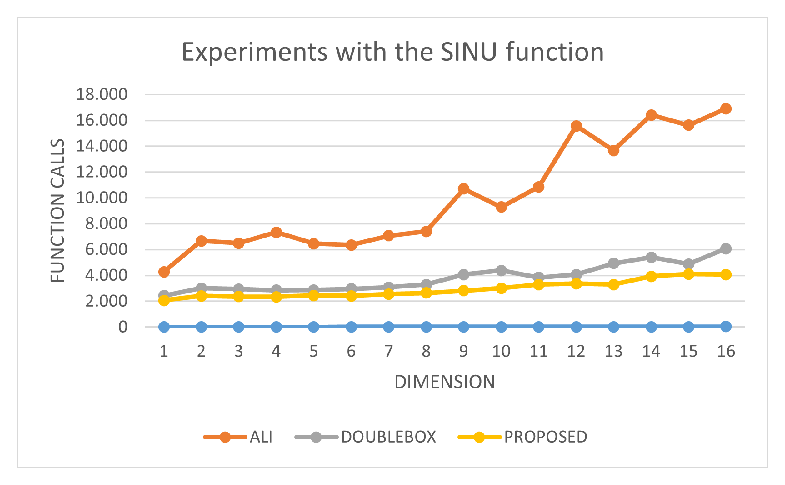
\includegraphics[scale=0.75]{sinu_plot_ipso}
\end{figure}


\section{Conclusions\label{sec:Conclusions}}

In the current work, three new modifications of the PSO method for
locating the global minimum of continuous and differentiable functions
were presented. The first modification alters the population velocity
calculation in an attempt to cause large changes in velocity when
the method is in its infancy and constantly finds new local minima
and small velocity changes when the method is to be centered around
a promising area of a global minimum. The second modification limits
the number of local searches performed by the method through an asymptotic
criterion based on derivative computation. The third modification
introduces a new termination criterion based on the observation that
the method from some iteration onwards will not be able to detect
a new minimum and therefore its termination should be considered.
All of these modifications have low computational requirements.

The experimental results showed that the second and third modifications
drastically reduce the required number of function calls without affecting
the performance of the method. In addition, the first modification
reduces the number of required calls, but only when the criterion
for avoiding local minimization is not present. 
\begin{thebibliography}{10}
\bibitem{go_physics1}L. Yang, D. Robin, F. Sannibale, C. Steier,
W. Wan, Global optimization of an accelerator lattice using multiobjective
genetic algorithms, Nuclear Instruments and Methods in Physics Research
Section A: Accelerators, Spectrometers, Detectors and Associated Equipment
\textbf{609}, pp. 50-57, 2009.

\bibitem{go_physics2}E. Iuliano, Global optimization of benchmark
aerodynamic cases using physics-based surrogate models, Aerospace
Science and Technology \textbf{67}, pp.273-286, 2017.

\bibitem{go_physics3}Q. Duan, S. Sorooshian, V. Gupta, Effective
and efficient global optimization for conceptual rainfall-runoff models,
Water Resources Research \textbf{28}, pp. 1015-1031 , 1992.

\bibitem{go_chem1}S. Heiles, R. L. Johnston, Global optimization
of clusters using electronic structure methods, Int. J. Quantum Chem.
\textbf{113}, pp. 2091-- 2109, 2013.

\bibitem{go_chem2}W.H. Shin, J.K. Kim, D.S. Kim, C. Seok, GalaxyDock2:
Protein--ligand docking using beta-complex and global optimization,
J. Comput. Chem. \textbf{34}, pp. 2647-- 2656, 2013.

\bibitem{go_chem3}A. Liwo, J. Lee, D.R. Ripoll, J. Pillardy, H. A.
Scheraga, Protein structure prediction by global optimization of a
potential energy function, Biophysics \textbf{96}, pp. 5482-5485,
1999.

\bibitem{go_econ1}Zwe-Lee Gaing, Particle swarm optimization to solving
the economic dispatch considering the generator constraints, IEEE
Transactions on \textbf{18} Power Systems, pp. 1187-1195, 2003.

\bibitem{go_econ2}C. D. Maranas, I. P. Androulakis, C. A. Floudas,
A. J. Berger, J. M. Mulvey, Solving long-term financial planning problems
via global optimization, Journal of Economic Dynamics and Control
\textbf{21}, pp. 1405-1425, 1997.

\bibitem{go_med1}Eva K. Lee, Large-Scale Optimization-Based Classification
Models in Medicine and Biology, Annals of Biomedical Engineering \textbf{35},
pp 1095-1109, 2007.

\bibitem{go_med2}Y. Cherruault, Global optimization in biology and
medicine, Mathematical and Computer Modelling \textbf{20}, pp. 119-132,
1994.

\bibitem{interval1}M.A. Wolfe, Interval methods for global optimization,
Applied Mathematics and Computation \textbf{75}, pp. 179-206, 1996.

\bibitem{interval2}T. Csendes and D. Ratz, Subdivision Direction
Selection in Interval Methods for Global Optimization, SIAM J. Numer.
Anal. \textbf{34}, pp. 922--938, 1997. 

\bibitem{crs1}W. L. Price, Global optimization by controlled random
search, Journal of Optimization Theory and Applications \textbf{40},
pp. 333-348, 1983.

\bibitem{crs2}Ivan K\v{r}iv�, Josef Tvrd�k, The controlled random
search algorithm in optimizing regression models, Computational Statistics
\& Data Analysis \textbf{20}, pp. 229-234, 1995.

\bibitem{crs3}M.M. Ali, A. T�rn, and S. Viitanen, A Numerical Comparison
of Some Modified Controlled Random Search Algorithms, Journal of Global
Optimization \textbf{11},pp. 377--385,1997.

\bibitem{simann_major}S. Kirkpatrick, CD Gelatt, , MP Vecchi, Optimization
by simulated annealing, Science \textbf{220}, pp. 671-680, 1983.

\bibitem{simann1}L. Ingber, Very fast simulated re-annealing, Mathematical
and Computer Modelling \textbf{12}, pp. 967-973, 1989.

\bibitem{simann2}R.W. Eglese, Simulated annealing: A tool for operational
research, Simulated annealing: A tool for operational research \textbf{46},
pp. 271-281, 1990.

\bibitem{diffe1}R. Storn, K. Price, Differential Evolution - A Simple
and Efficient Heuristic for Global Optimization over Continuous Spaces,
Journal of Global Optimization \textbf{11}, pp. 341-359, 1997.

\bibitem{diffe2}J. Liu, J. Lampinen, A Fuzzy Adaptive Differential
Evolution Algorithm. Soft Comput \textbf{9}, pp.448--462, 2005.

\bibitem{pso_major}J. Kennedy and R. Eberhart, \textquotedbl Particle
swarm optimization,\textquotedbl{} Proceedings of ICNN'95 - International
Conference on Neural Networks, 1995, pp. 1942-1948 vol.4, doi: 10.1109/ICNN.1995.488968.

\bibitem{pso1}Riccardo Poli, James Kennedy kennedy, Tim Blackwell,
Particle swarm optimization An Overview, Swarm Intelligence \textbf{1},
pp 33-57, 2007. 

\bibitem{pso2}Ioan Cristian Trelea, The particle swarm optimization
algorithm: convergence analysis and parameter selection, Information
Processing Letters \textbf{85}, pp. 317-325, 2003.

\bibitem{aco1}M. Dorigo, M. Birattari and T. Stutzle, Ant colony
optimization, IEEE Computational Intelligence Magazine \textbf{1},
pp. 28-39, 2006.

\bibitem{aco2}K. Socha, M. Dorigo, Ant colony optimization for continuous
domains, European Journal of Operational Research 185, pp. 1155-1173,
2008.

\bibitem{ga1}D. Goldberg, Genetic Algorithms in Search, Optimization
and Machine Learning, Addison-Wesley Publishing Company, Reading,
Massachussets, 1989.

\bibitem{ga2}Z. Michaelewicz, Genetic Algorithms + Data Structures
= Evolution Programs. Springer - Verlag, Berlin, 1996.

\bibitem{ga3}S.A. Grady, M.Y. Hussaini, M.M. Abdullah, Placement
of wind turbines using genetic algorithms, Renewable Energy \textbf{30},
pp. 259-270, 2005.

\bibitem{gpu1}Y. Zhou and Y. Tan, \textquotedbl GPU-based parallel
particle swarm optimization,\textquotedbl{} 2009 IEEE Congress on
Evolutionary Computation, pp. 1493-1500, 2009.

\bibitem{gpu2}L. Dawson and I. Stewart, \textquotedbl Improving
Ant Colony Optimization performance on the GPU using CUDA,\textquotedbl{}
2013 IEEE Congress on Evolutionary Computation, 2013, pp. 1901-1908,
doi: 10.1109/CEC.2013.6557791.

\bibitem{gpu3}Barkalov, K., Gergel, V. Parallel global optimization
on GPU. J Glob Optim 66, 3--20 (2016). 

\bibitem{psophysics1}Anderson Alvarenga de Moura Meneses, Marcelo
Dornellas, Machado Roberto Schirru, Particle Swarm Optimization applied
to the nuclear reload problem of a Pressurized Water Reactor, Progress
in Nuclear Energy \textbf{51}, pp. 319-326, 2009.

\bibitem{psophysics2}Ranjit Shaw, Shalivahan Srivastava, Particle
swarm optimization: A new tool to invert geophysical data, Geophysics
\textbf{72}, 2007.

\bibitem{psochem1}C. O. Ourique, E.C. Biscaia, J.C. Pinto, The use
of particle swarm optimization for dynamical analysis in chemical
processes, Computers \& Chemical Engineering \textbf{26}, pp. 1783-1793,
2002.

\bibitem{psochem2}H. Fang, J. Zhou, Z. Wang et al, Hybrid method
integrating machine learning and particle swarm optimization for smart
chemical process operations, Front. Chem. Sci. Eng. \textbf{16}, pp.
274--287, 2022.

\bibitem{psomed1}M.P. Wachowiak, R. Smolikova, Yufeng Zheng, J.M.
Zurada, A.S. Elmaghraby, An approach to multimodal biomedical image
registration utilizing particle swarm optimization, IEEE Transactions
on Evolutionary Computation \textbf{8}, pp. 289-301, 2004.

\bibitem{psomed2}Yannis Marinakis. Magdalene Marinaki, Georgios Dounias,
Particle swarm optimization for pap-smear diagnosis, Expert Systems
with Applications \textbf{35}, pp. 1645-1656, 2008. 

\bibitem{psoecon}Jong-Bae Park, Yun-Won Jeong, Joong-Rin Shin, Kwang
Y. Lee, An Improved Particle Swarm Optimization for Nonconvex Economic
Dispatch Problems, IEEE Transactions on Power Systems \textbf{25},
pp. 156-16\textbf{216}6, 2010.

\bibitem{pso_mutation1}A. Stacey, M. Jancic, I. Grundy, Particle
swarm optimization with mutation, In: 2003 Congress on Evolutionary
Computation, 2003. CEC '03., pp. 1425-1430, 2003.

\bibitem{pso_mutation2}M. Pant, R. Thangaraj, A. Abraham, Particle
Swarm Optimization Using Adaptive Mutation, In: 2008 19th International
Workshop on Database and Expert Systems Applications, pp. 519-523,
2008.

\bibitem{pso_mutation3}N. Higashi, H. Iba, Particle swarm optimization
with Gaussian mutation, In: Proceedings of the 2003 IEEE Swarm Intelligence
Symposium. SIS'03 (Cat. No.03EX706), pp. 72-79, 2003.

\bibitem{pso_initvelocity}A. Engelbrecht, \textquotedbl Particle
swarm optimization: Velocity initialization,\textquotedbl{} 2012 IEEE
Congress on Evolutionary Computation, pp. 1-8, 2012.

\bibitem{psohybrid1}B. Liu, L. Wang, Y.H. Jin, F. Tang, D.X. Huang,
Improved particle swarm optimization combined with chaos, Chaos Solitons
and Fractals \textbf{25}, pp. 1261-1271, 2005.

\bibitem{psohybrid2}X.H. Shi, Y.C. Liang, H.P. Lee, C. Lu, L.M. Wang,
An improved GA and a novel PSO-GA based hybrid algorithm, Information
Processing Letters \textbf{93}, pp. 255-261, 2005.

\bibitem{psohybrid3}Harish Garg, A hybrid PSO-GA algorithm for constrained
optimization problems, Applied Mathematics and Computation \textbf{274},
pp. 292-305, 2016.

\bibitem{pso_parallel1}J. F. Schutte, J. A. Reinbolt, B. J. Fregly,
R. T. Haftka, A. D. George, Parallel global optimization with the
particle swarm algorithm, Int. J. Numer. Meth. Engng. \textbf{61},
pp. 2296-2315, 2004.

\bibitem{pso_parallel2}B-Il Koh, A.D. George, R.T. Haftka, B.J. Fregly,
Parallel asynchronous particle swarm optimization. Int. J. Numer.
Meth. Engng., \textbf{67}, pp. 578-595, 2006.

\bibitem{pso_parallel3}G. Venter, J. Sobieszczanski-Sobieski, Parallel
Particle Swarm Optimization Algorithm Accelerated by Asynchronous
Evaluations, Journal of Aerospace Computing, Information, and Communication
\textbf{3}, pp. 123-137, 2006.

\bibitem{pso_velocity1}Z.L. Gaing, Particle swarm optimization to
solving the economic dispatch considering the generator constraints,
IEEE Transactions on Power Systems \textbf{18}, pp. 1187-1195, 2003.

\bibitem{pso_velocity2}X. Yang, Jinsha Yuan, Jiangy Yuan, H. Mao,
A modified particle swarm optimizer with dynamic adaptation, Applied
Mathematics and Computation \textbf{189}, pp. 1205-1213, 2007.

\bibitem{pso_velocity3}Y. Jiang, T. Hu, C. Huang, X. Wu, An improved
particle swarm optimization algorithm, Applied Mathematics and Computation
\textbf{193}, pp. 231-239, 2007.

\bibitem{random_inertia}R.C. Eberhart, Y.H. Shi, Tracking and optimizing
dynamic systems with particle swarms, in: Congress on Evolutionary
Computation, Korea, 2001.

\bibitem{inertia1} Y.H. Shi, R.C. Eberhart, Empirical study of particle
swarm optimization, in: Congress on Evolutionary Computation, Washington
DC, USA, 1999. 

\bibitem{inertia2}Y.H. Shi, R.C. Eberhart, Experimental study of
particle swarm optimization, in: SCI2000 Conference, Orlando, 2000.

\bibitem{inertia3}Y. Zheng, L. Ma, L. Zhang, J. Qian, Empirical study
of particle swarm optimizer with an increasing inertia weight, in:
IEEE Congress on Evolutionary Computation, 2003.

\bibitem{inertia4}Y. Zheng, L. Ma, L. Zhang, J. Qian, On the convergence
analysis and param- eter selection in particle swarm optimization,
in: Proceedings of the Second International Conference on Machine
Learning and Cybernetics, 2003.

\bibitem{minfinder}Ioannis G. Tsoulos, Isaac E. Lagaris, MinFinder:
Locating all the local minima of a function, Computer Physics Communications
\textbf{174}, pp. 166-179, 2006.

\bibitem{AliKaelo}M.M. Ali, P. Kaelo, Improved particle swarm algorithms
for global optimization, Applied Mathematics and Computation \textbf{196},
pp. 578--593, 2008.

\bibitem{doublepop_tsoulos}I.G. Tsoulos, Modifications of real code
genetic algorithm for global optimization, Applied Mathematics and
Computation \textbf{203}, pp. 598-607, 2008.

\bibitem{Ali1}M. Montaz Ali, Charoenchai Khompatraporn, Zelda B.
Zabinsky, A Numerical Evaluation of Several Stochastic Algorithms
on Selected Continuous Global Optimization Test Problems, Journal
of Global Optimization \textbf{31}, pp 635-672, 2005. 

\bibitem{Floudas1}C.A. Floudas, P.M. Pardalos, C. Adjiman, W. Esposoto,
Z. G$\ddot{\mbox{u}}$m$\ddot{\mbox{u}}$s, S. Harding, J. Klepeis,
C. Meyer, C. Schweiger, Handbook of Test Problems in Local and Global
Optimization, Kluwer Academic Publishers, Dordrecht, 1999.

\bibitem{testfunctions1}M.M. Ali and P. Kaelo, Improved particle
swarm algorithms for global optimization, Applied Mathematics and
Computation \textbf{196}, pp. 578-593, 2008.

\bibitem{testfunctions2}H. Koyuncu, R. Ceylan, A PSO based approach:
Scout particle swarm algorithm for continuous global optimization
problems, Journal of Computational Design and Engineering \textbf{6},
pp. 129--142, 2019.

\bibitem{testfunctions3}Patrick Siarry, G�rard Berthiau, Fran�ois
Durdin, Jacques Haussy, ACM Transactions on Mathematical Software
\textbf{23}, pp 209--228, 1997.

\bibitem{testfunctions4}I.G. Tsoulos, I.E. Lagaris, GenMin: An enhanced
genetic algorithm for global optimization, Computer Physics Communications\textbf{
178, }pp. 843-851, 2008.

\bibitem{Powell}M.J.D Powell, A Tolerant Algorithm for Linearly Constrained
Optimization Calculations, Mathematical Programming \textbf{45}, pp.
547-566, 1989. 

\bibitem{gkls}M. Gaviano, D.E. Ksasov, D. Lera, Y.D. Sergeyev, Software
for generation of classes of test functions with known local and global
minima for global optimization, ACM Trans. Math. Softw. \textbf{29},
pp. 469-480, 2003.

\bibitem{Jones}J.E. Lennard-Jones, On the Determination of Molecular
Fields, Proc. R. Soc. Lond. A \textbf{ 106}, pp. 463--477, 1924.
\end{thebibliography}

\end{document}
